\documentclass[border=4pt]{standalone}
% Shared typography and colours for the standalone figures.
\usepackage{unicode-math}
\setmainfont{TeX Gyre Termes}
\setmathfont{TeX Gyre Termes Math}
\usepackage{tikz}
\usetikzlibrary{arrows.meta,positioning,calc,decorations.pathreplacing}
\usepackage{pgfplots}
\pgfplotsset{compat=1.18}

% One colour per element or subsystem. Record the mapping in
% the working repository conventions and use it identically in every figure.
\definecolor{elemA}{HTML}{1F5FA8}
\definecolor{elemB}{HTML}{B8461B}
\definecolor{elemC}{HTML}{2E7D32}
\definecolor{elemD}{HTML}{6A4C93}
\definecolor{frameline}{HTML}{555555}

% Article-specific diagram styling; common figure-style.tex remains managed.
\usepackage{circuitikz}
\usetikzlibrary{decorations.pathmorphing,fit,backgrounds}
\tikzset{
  every node/.style={font=\small},
  block/.style={draw=frameline,rounded corners=2pt,minimum height=7mm,align=center,fill=white},
  massA/.style={draw=elemA,fill=elemA!10,thick},
  massB/.style={draw=elemB,fill=elemB!10,thick},
  receiver/.style={draw=elemC,fill=elemC!9,thick},
  mediator/.style={draw=elemD,fill=elemD!8,thick},
  flow/.style={-{Latex[length=2.3mm]},thick},
  boundary/.style={draw=frameline,dashed,rounded corners=3pt},
  spring/.style={decorate,decoration={coil,aspect=.4,segment length=3mm,amplitude=1.5mm},thick,elemD}
}

\begin{document}
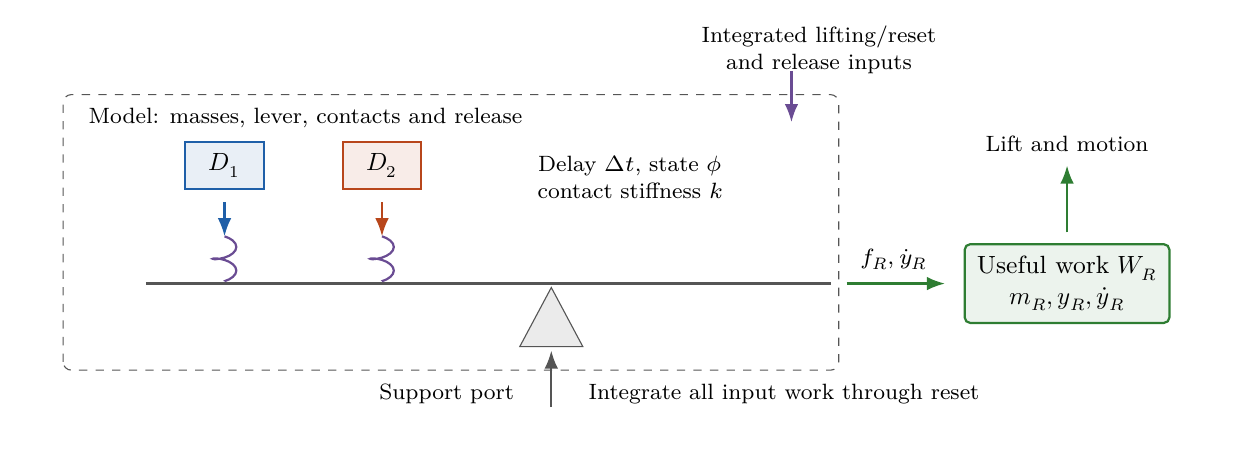
\begin{tikzpicture}
\path[use as bounding box] (0,-.65) rectangle (15,4.4);
\draw[boundary] (.45,.05) rectangle (10.3,3.55);
\node[anchor=north west,font=\footnotesize] at (.65,3.5) {Model: masses, lever, contacts and release};
\node[font=\footnotesize,align=center] at (10.05,4.12) {Integrated lifting/reset\\and release inputs};
\draw[flow,elemD] (9.7,3.85)--(9.7,3.2);
\draw[frameline,very thick] (1.5,1.15)--(10.2,1.15);
\draw[frameline,fill=frameline!12] (6.65,1.1)--(6.25,.35)--(7.05,.35)--cycle;
\draw[massA] (2,2.35) rectangle (3,2.95);
\draw[massB] (4,2.35) rectangle (5,2.95);
\node at (2.5,2.65) {$D_1$};
\node at (4.5,2.65) {$D_2$};
\draw[flow,elemA] (2.5,2.18)--(2.5,1.75);
\draw[flow,elemB] (4.5,2.18)--(4.5,1.75);
\draw[spring] (2.5,1.75)--(2.5,1.18);
\draw[spring] (4.5,1.75)--(4.5,1.18);
\node[font=\footnotesize,align=center] at (7.65,2.5) {Delay $\Delta t$, state $\phi$\\contact stiffness $k$};
\draw[flow,elemC] (10.4,1.15)--(11.65,1.15);
\node[font=\footnotesize,above] at (11.0,1.2) {$f_R,\dot y_R$};
\node[block,receiver,minimum width=2.6cm,minimum height=1cm] at (13.2,1.15) {Useful work $W_R$\\$m_R,y_R,\dot y_R$};
\draw[flow,elemC] (13.2,1.8)--(13.2,2.65);
\node[anchor=south,font=\footnotesize] at (13.2,2.7) {Lift and motion};
\draw[flow,frameline] (6.65,-.42)--(6.65,.3);
\node[font=\footnotesize,anchor=east] at (6.3,-.25) {Support port};
\node[font=\footnotesize,anchor=west] at (7.0,-.25) {Integrate all input work through reset};
\end{tikzpicture}
\end{document}
